\documentclass[aspectratio=169]{ctexbeamer}
\usetheme{Madrid}
\usecolortheme{default}
\setbeamertemplate{navigation symbols}{}

\usepackage{amsmath}
\usepackage{amssymb}
\usepackage{array}
\usepackage{booktabs}
\usepackage{fancyvrb}
\usepackage{graphicx}
\usepackage{hyperref}
\usepackage{tikz}
\usepackage{xcolor}
\usetikzlibrary{positioning}

\definecolor{PrimaryBlue}{RGB}{28,74,118}
\definecolor{AccentTeal}{RGB}{42,157,143}
\definecolor{AccentOrange}{RGB}{231,111,81}
\definecolor{SoftGray}{RGB}{245,247,250}
\definecolor{CodeGray}{RGB}{78,78,78}

\setbeamercolor{structure}{fg=PrimaryBlue}
\setbeamercolor{frametitle}{fg=PrimaryBlue}
\setbeamercolor{title}{fg=white,bg=PrimaryBlue}
\setbeamercolor{titlelike}{fg=white,bg=PrimaryBlue}
\setbeamercolor{subtitle}{fg=white}
\setbeamercolor{block title}{fg=white,bg=PrimaryBlue}
\setbeamercolor{block body}{bg=black!3}
\setbeamercolor{alerted text}{fg=AccentOrange}

\DefineVerbatimEnvironment{CodeBlock}{Verbatim}{
  fontsize=\scriptsize,
  frame=single,
  framesep=2mm,
  numbers=left,
  numbersep=4pt
}

\title{Python資料分析跟機器學習}
\subtitle{Twitter 情緒分析期末專題報告}
\author{製作人 B12204033 施卲}
\institute{期末專題簡報}
\date{2026年6月12日}

\begin{document}

\begin{frame}[plain]
\centering
\vspace{1.1cm}
{\color{PrimaryBlue}\bfseries\LARGE Python資料分析跟機器學習\par}
\vspace{0.4cm}
{\large Twitter 情緒分析期末專題報告\par}
\vspace{1.0cm}
\begin{beamercolorbox}[wd=0.82\paperwidth, rounded=true, shadow=true, sep=12pt, center]{block title}
製作人 B12204033 施卲
\end{beamercolorbox}
\vspace{0.9cm}
{\large 期末專題簡報\par}
\vspace{0.8cm}
{\Large 2026 年 6 月 12 日\par}
\end{frame}

\begin{frame}{報告大綱}
\tableofcontents
\end{frame}

\section{專題介紹}

\begin{frame}{研究背景與動機}
\begin{itemize}
  \item 社群媒體在公共議題傳播中具有即時、密集且可量化的特性。
  \item Twitter 貼文可作為觀察民眾情緒變化的重要資料來源。
  \item 本專題希望以 Python 建立一套完整流程，從資料清理、情緒分析到視覺化輸出。
  \item 目標不只在於得到結果，也要讓分析程式具備可重跑、可維護與可展示的特性。
\end{itemize}
\end{frame}

\begin{frame}{專題目標與研究問題}
\begin{block}{專題目標}
建立一個可重複執行的 Twitter 情緒分析流程，並輸出適合期末報告展示的圖表與摘要報表。
\end{block}

\vspace{0.5em}
\begin{itemize}
  \item 如何清理大量推文文字，保留可分析的語意資訊？
  \item 如何以 VADER 模型為基礎，將推文分類為正向、中立、負向？
  \item 如何觀察情緒比例在不同時間區段的變化？
  \item 如何讓最終成果兼具分析價值與簡報可讀性？
\end{itemize}
\end{frame}

\begin{frame}{專題流程總覽}
\centering
\begin{tikzpicture}[node distance=1.25cm, >=latex, rounded corners]
  \node[draw, fill=PrimaryBlue!8, minimum width=2.2cm, minimum height=0.95cm] (raw) {原始 CSV};
  \node[draw, fill=PrimaryBlue!8, minimum width=2.2cm, minimum height=0.95cm, right=of raw] (load) {資料載入};
  \node[draw, fill=PrimaryBlue!8, minimum width=2.2cm, minimum height=0.95cm, right=of load] (clean) {文字清理};
  \node[draw, fill=PrimaryBlue!8, minimum width=2.2cm, minimum height=0.95cm, right=of clean] (sent) {情緒判定};
  \node[draw, fill=PrimaryBlue!8, minimum width=2.2cm, minimum height=0.95cm, below=of clean] (agg) {時間聚合};
  \node[draw, fill=PrimaryBlue!8, minimum width=2.2cm, minimum height=0.95cm, left=of agg] (report) {CSV 報表};
  \node[draw, fill=PrimaryBlue!8, minimum width=2.2cm, minimum height=0.95cm, right=of agg] (fig) {圖形輸出};

  \draw[->, thick] (raw) -- (load);
  \draw[->, thick] (load) -- (clean);
  \draw[->, thick] (clean) -- (sent);
  \draw[->, thick] (sent) -- (agg);
  \draw[->, thick] (agg) -- (report);
  \draw[->, thick] (agg) -- (fig);
\end{tikzpicture}

\vspace{1em}
\begin{itemize}
  \item 核心流程集中於 \texttt{twitter\_sentiment\_project/} 套件。
  \item 最終輸出包含分析圖、關鍵字圖、主題分布圖與多份 CSV 摘要。
\end{itemize}
\end{frame}

\section{資料與系統設計}

\begin{frame}{資料來源與資料特徵}
\begin{columns}[T]
  \begin{column}{0.52\textwidth}
    \begin{block}{資料概況}
    \begin{itemize}
      \item 原始資料筆數：82,309
      \item 有效分析筆數：82,035
      \item 無效或重複資料移除：274
      \item 分析日期：2021-01-06
      \item 主要欄位：\texttt{tweet\_id}、\texttt{query}、\texttt{text}、\texttt{created\_at}
    \end{itemize}
    \end{block}
  \end{column}
  \begin{column}{0.44\textwidth}
    \begin{block}{資料特性}
    \begin{itemize}
      \item 屬於混合主題資料集
      \item 每個 query 的筆數相近
      \item 適合用於比較整體情緒與時間變化
      \item 需先完成欄位驗證與時間格式轉換
    \end{itemize}
    \end{block}
  \end{column}
\end{columns}
\end{frame}

\begin{frame}{專案架構重整}
\begin{columns}[T]
  \begin{column}{0.52\textwidth}
    \begin{block}{主要資料夾}
\small
\begin{tabular}{>{\ttfamily}p{0.42\linewidth} p{0.48\linewidth}}
data/raw & 原始資料 \\
data/processed & 清理後資料 \\
outputs/figures & 圖形成果 \\
outputs/reports & 分析報表 \\
slides & 簡報檔案 \\
\end{tabular}
    \end{block}
  \end{column}
  \begin{column}{0.44\textwidth}
    \begin{block}{核心模組}
\scriptsize
\begin{tabular}{>{\ttfamily}p{0.52\linewidth} p{0.34\linewidth}}
data\_loader.py & 載入資料 \\
preprocessor.py & 清理文字 \\
sentiment\_analyzer.py & 情緒評分 \\
analyzer.py & 聚合與摘要 \\
visualizer.py & 圖表繪製 \\
pipeline.py & 串接流程 \\
\end{tabular}
    \end{block}
  \end{column}
\end{columns}
\end{frame}

\begin{frame}{執行環境與套件選擇}
\begin{columns}[T]
  \begin{column}{0.48\textwidth}
    \begin{block}{主要技術}
    \begin{itemize}
      \item Python 3
      \item pandas
      \item matplotlib
      \item vaderSentiment
      \item LaTeX Beamer
    \end{itemize}
    \end{block}
  \end{column}
  \begin{column}{0.48\textwidth}
    \begin{block}{設計理由}
    \begin{itemize}
      \item pandas 處理大量表格資料穩定
      \item VADER 適合短文字情緒分析
      \item matplotlib 可輸出高解析度 PNG
      \item Beamer 適合正式學術簡報
    \end{itemize}
    \end{block}
  \end{column}
\end{columns}
\end{frame}

\section{核心程式碼講解}

\begin{frame}[fragile]{程式碼一：資料載入與欄位驗證}
\begin{CodeBlock}
def load_data(file_path=None):
    path = Path(file_path) if file_path else resolve_default_input_file()
    df = pd.read_csv(path)
    prepared = df.copy()
    prepared["text"] = prepared["text"].astype(str)
    prepared["created_at"] = pd.to_datetime(
        prepared["created_at"], errors="coerce", utc=True
    )
    prepared = prepared.dropna(subset=["created_at", "text"]).copy()
    prepared = prepared.drop_duplicates(subset=["tweet_id"])
    return prepared.sort_values("created_at").reset_index(drop=True)
\end{CodeBlock}

\begin{itemize}
  \item 先確認資料路徑，再讀取 CSV。
  \item 將 \texttt{created\_at} 統一轉換為可排序的時間格式。
  \item 刪除空值與重複資料，確保後續統計一致。
\end{itemize}
\end{frame}

\begin{frame}[fragile]{程式碼二：文字清理與斷詞}
\begin{CodeBlock}
def clean_tweet(text):
    normalized = html.unescape(str(text)).replace("\n", " ")
    normalized = URL_PATTERN.sub(" ", normalized)
    normalized = MENTION_PATTERN.sub(" ", normalized)
    normalized = normalized.replace("#", " ").lower()
    normalized = NON_TEXT_PATTERN.sub(" ", normalized)
    return MULTISPACE_PATTERN.sub(" ", normalized).strip()

def apply_cleaning(df):
    cleaned = df.copy()
    cleaned["clean_text"] = cleaned["text"].apply(clean_tweet)
    cleaned["tokens"] = cleaned["clean_text"].apply(tokenize)
    cleaned["token_count"] = cleaned["tokens"].apply(len)
    return cleaned
\end{CodeBlock}

\begin{itemize}
  \item 移除網址、帳號提及、特殊符號與多餘空白。
  \item 將推文轉為小寫，提升情緒分析與關鍵詞統計的一致性。
  \item 額外保留 \texttt{tokens} 與 \texttt{token\_count} 供後續分析使用。
\end{itemize}
\end{frame}

\begin{frame}[fragile]{程式碼三：情緒分數與標籤判定}
\begin{CodeBlock}
def get_sentiment_score(text):
    analyzer = get_sentiment_analyzer()
    return analyzer.polarity_scores(text)["compound"]

def label_sentiment(score, positive_threshold=0.05, negative_threshold=-0.05):
    if score >= positive_threshold:
        return "Positive"
    if score <= negative_threshold:
        return "Negative"
    return "Neutral"

def apply_sentiment(df):
    analyzed = df.copy()
    analyzed["sentiment_score"] = analyzed["clean_text"].apply(get_sentiment_score)
    analyzed["sentiment"] = analyzed["sentiment_score"].apply(label_sentiment)
    return analyzed
\end{CodeBlock}

\scriptsize
\begin{itemize}
  \item VADER 適合用來評估短文字情緒分數。
  \item 本專題以固定門檻區分正向、中立與負向。
  \item 快取機制可避免重複初始化分析器。
\end{itemize}
\end{frame}

\begin{frame}[fragile]{程式碼四：時間區段聚合}
\begin{CodeBlock}
def compute_time_sentiment(df, freq="15min", min_tweets=10):
    working = df.copy()
    working["time_bin"] = working["created_at"].dt.floor(freq)
    sentiment_counts = (
        working.groupby(["time_bin", "sentiment"])
        .size().unstack(fill_value=0)
        .reindex(columns=SENTIMENT_LABELS, fill_value=0)
    )
    sentiment_counts["tweet_count"] = sentiment_counts.sum(axis=1)
    for sentiment in SENTIMENT_LABELS:
        sentiment_counts[f"{sentiment}_ratio"] = (
            sentiment_counts[sentiment] / sentiment_counts["tweet_count"]
        )
    return sentiment_counts[sentiment_counts["tweet_count"] >= min_tweets]
\end{CodeBlock}

\begin{itemize}
  \item 以 15 分鐘為單位觀察情緒變化。
  \item 每個時間區段都會計算三種情緒的比例。
  \item 若推文數量過少，該區段會被排除以避免噪音影響。
\end{itemize}
\end{frame}

\begin{frame}[fragile]{程式碼五：管線整合與圖表輸出}
\begin{CodeBlock}
def run_pipeline(input_file=None, output_dir=OUTPUT_DIR, freq="15min"):
    raw_df = load_data(input_file)
    cleaned_df = apply_cleaning(raw_df)
    scored_df = apply_sentiment(cleaned_df)
    time_df = compute_time_sentiment(scored_df, freq=freq, min_tweets=10)
    distribution_df = compute_sentiment_distribution(scored_df)
    top_terms_df = compute_top_terms(scored_df, top_n=12)
    plot_sentiment_dashboard(time_df, distribution_df, summary_df, ...)
    plot_top_terms(top_terms_df, ...)
    plot_query_distribution(query_distribution_df, ...)
    return PipelineOutputs(...)
\end{CodeBlock}

\begin{itemize}
  \item \texttt{pipeline.py} 將所有分析步驟整合為一個可重跑的流程。
  \item 除了圖片之外，也同步輸出多份 CSV 報表。
  \item 這種設計能兼顧程式維護、報告撰寫與成果展示。
\end{itemize}
\end{frame}

\begin{frame}[fragile]{程式碼六：主程式入口與執行方式}
\begin{columns}[T]
  \begin{column}{0.54\textwidth}
\begin{CodeBlock}
def main():
    args = parse_args()
    outputs = run_pipeline(
        input_file=args.input,
        output_dir=args.output_dir,
        freq=args.freq,
        min_tweets=args.min_tweets,
        top_n_terms=args.top_n_terms,
    )
    print(f"Dashboard figure: {outputs.dashboard_path}")

if __name__ == "__main__":
    main()
\end{CodeBlock}
  \end{column}
  \begin{column}{0.42\textwidth}
    \begin{block}{執行指令}
\ttfamily\scriptsize
python3 main.py\\
python3 main.py --freq 15min\\
python3 main.py --top-n-terms 12
    \end{block}

    \begin{block}{意義}
    \begin{itemize}
      \item CLI 參數化提高彈性。
      \item 可快速調整時間粒度與輸出設定。
      \item 便於之後擴充為不同資料集版本。
    \end{itemize}
    \end{block}
  \end{column}
\end{columns}
\end{frame}

\section{分析成果}

\begin{frame}{輸出成果與檔案}
\begin{columns}[T]
  \begin{column}{0.50\textwidth}
    \begin{block}{圖形輸出}
    \begin{itemize}
      \item \texttt{sentiment\_dashboard.png}
      \item \texttt{top\_terms\_by\_sentiment.png}
      \item \texttt{query\_distribution.png}
    \end{itemize}
    \end{block}
  \end{column}
  \begin{column}{0.46\textwidth}
    \begin{block}{報表輸出}
    \begin{itemize}
      \item \texttt{overall\_summary.csv}
      \item \texttt{sentiment\_distribution.csv}
      \item \texttt{time\_sentiment\_summary.csv}
      \item \texttt{top\_terms\_by\_sentiment.csv}
    \end{itemize}
    \end{block}
  \end{column}
\end{columns}

\vspace{0.7em}
\begin{alertblock}{成果整理重點}
本專題的成果不只是一張圖，而是一組可重複產生的分析資產，方便用於書面報告、簡報與後續延伸研究。
\end{alertblock}
\end{frame}

\begin{frame}{情緒儀表板結果}
\centering
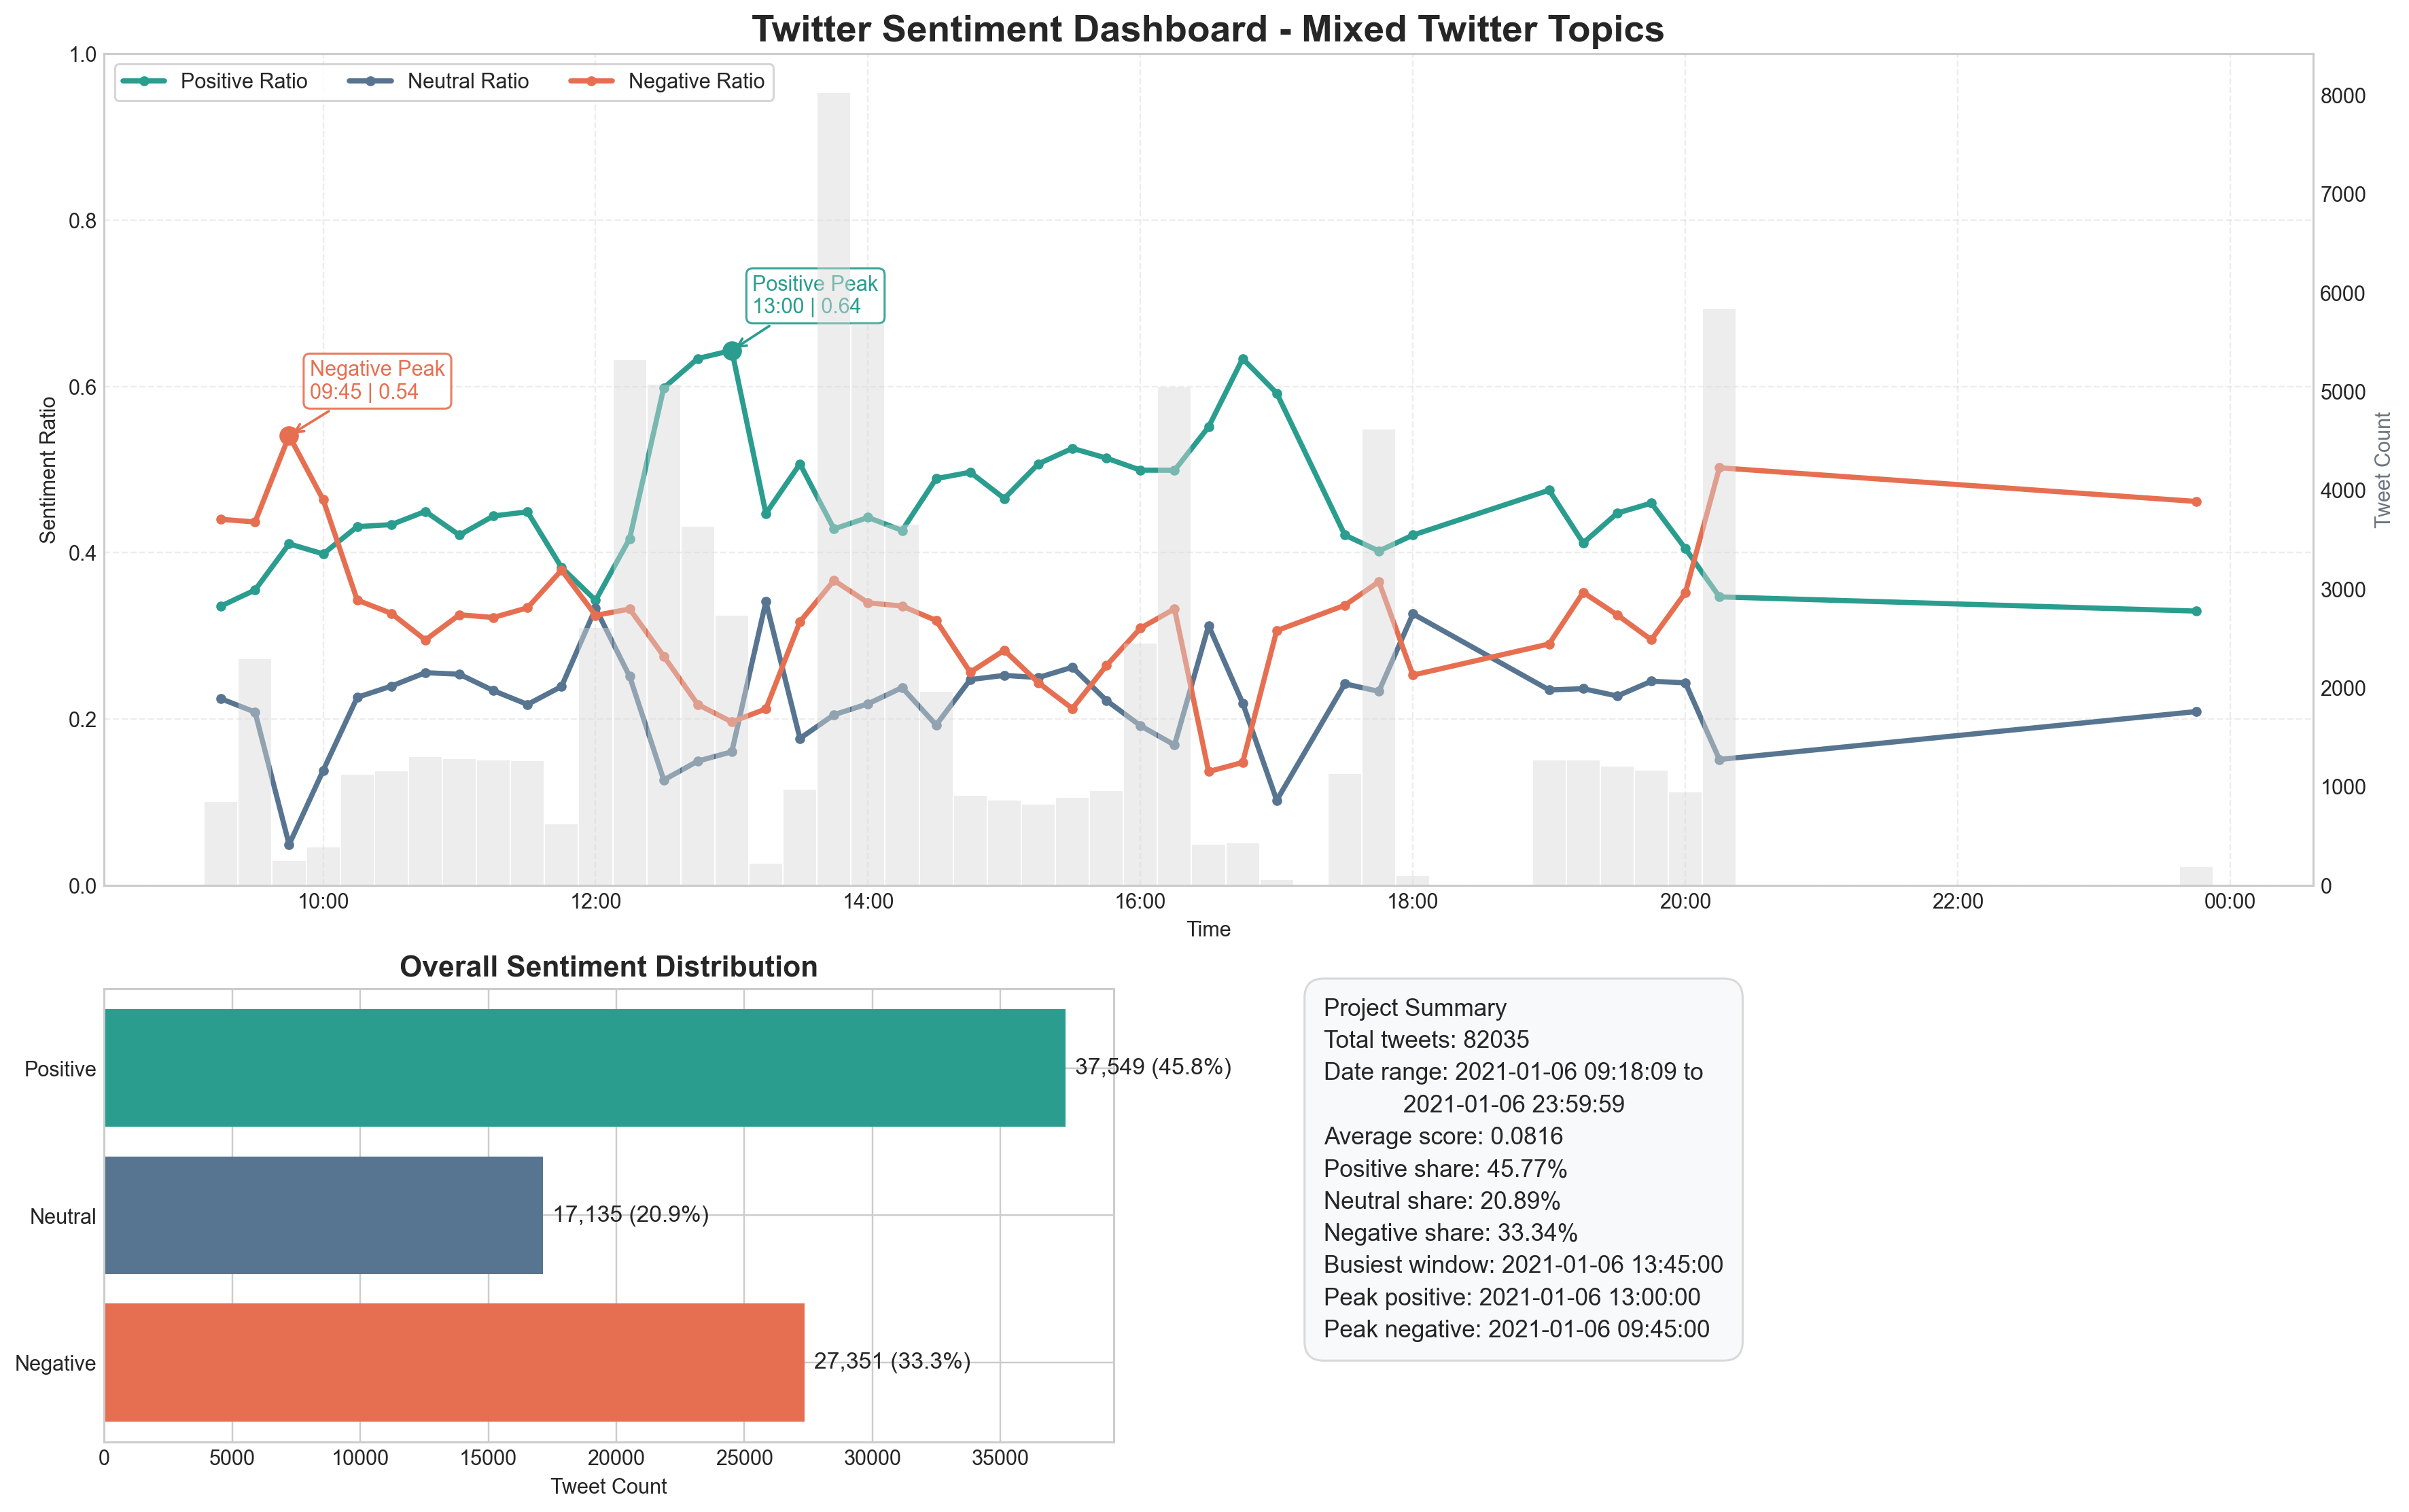
\includegraphics[width=0.93\linewidth,height=0.80\textheight,keepaspectratio]{../outputs/figures/sentiment_dashboard.png}
\end{frame}

\begin{frame}{關鍵詞分析結果}
\centering
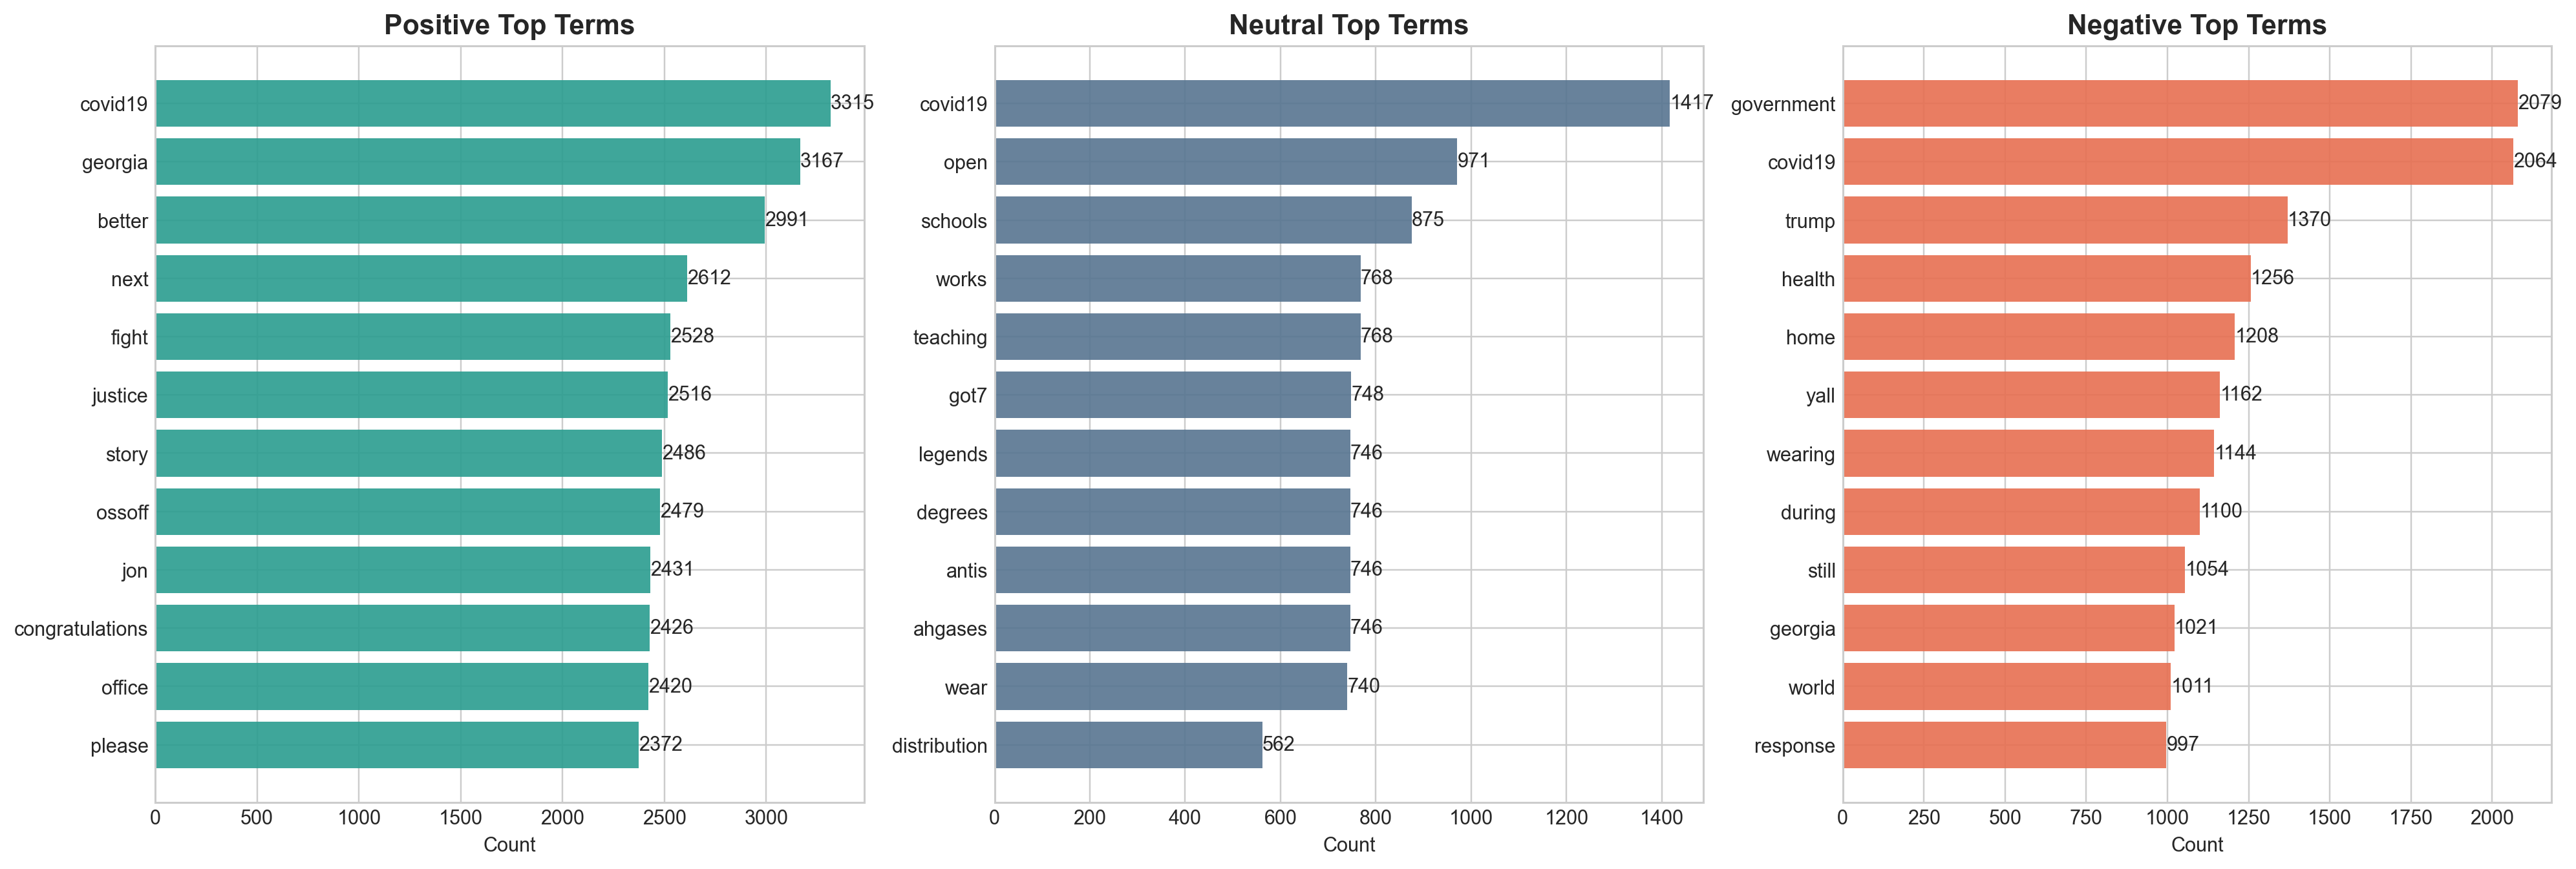
\includegraphics[width=0.95\linewidth,height=0.80\textheight,keepaspectratio]{../outputs/figures/top_terms_by_sentiment.png}
\end{frame}

\begin{frame}{主題分布結果}
\centering
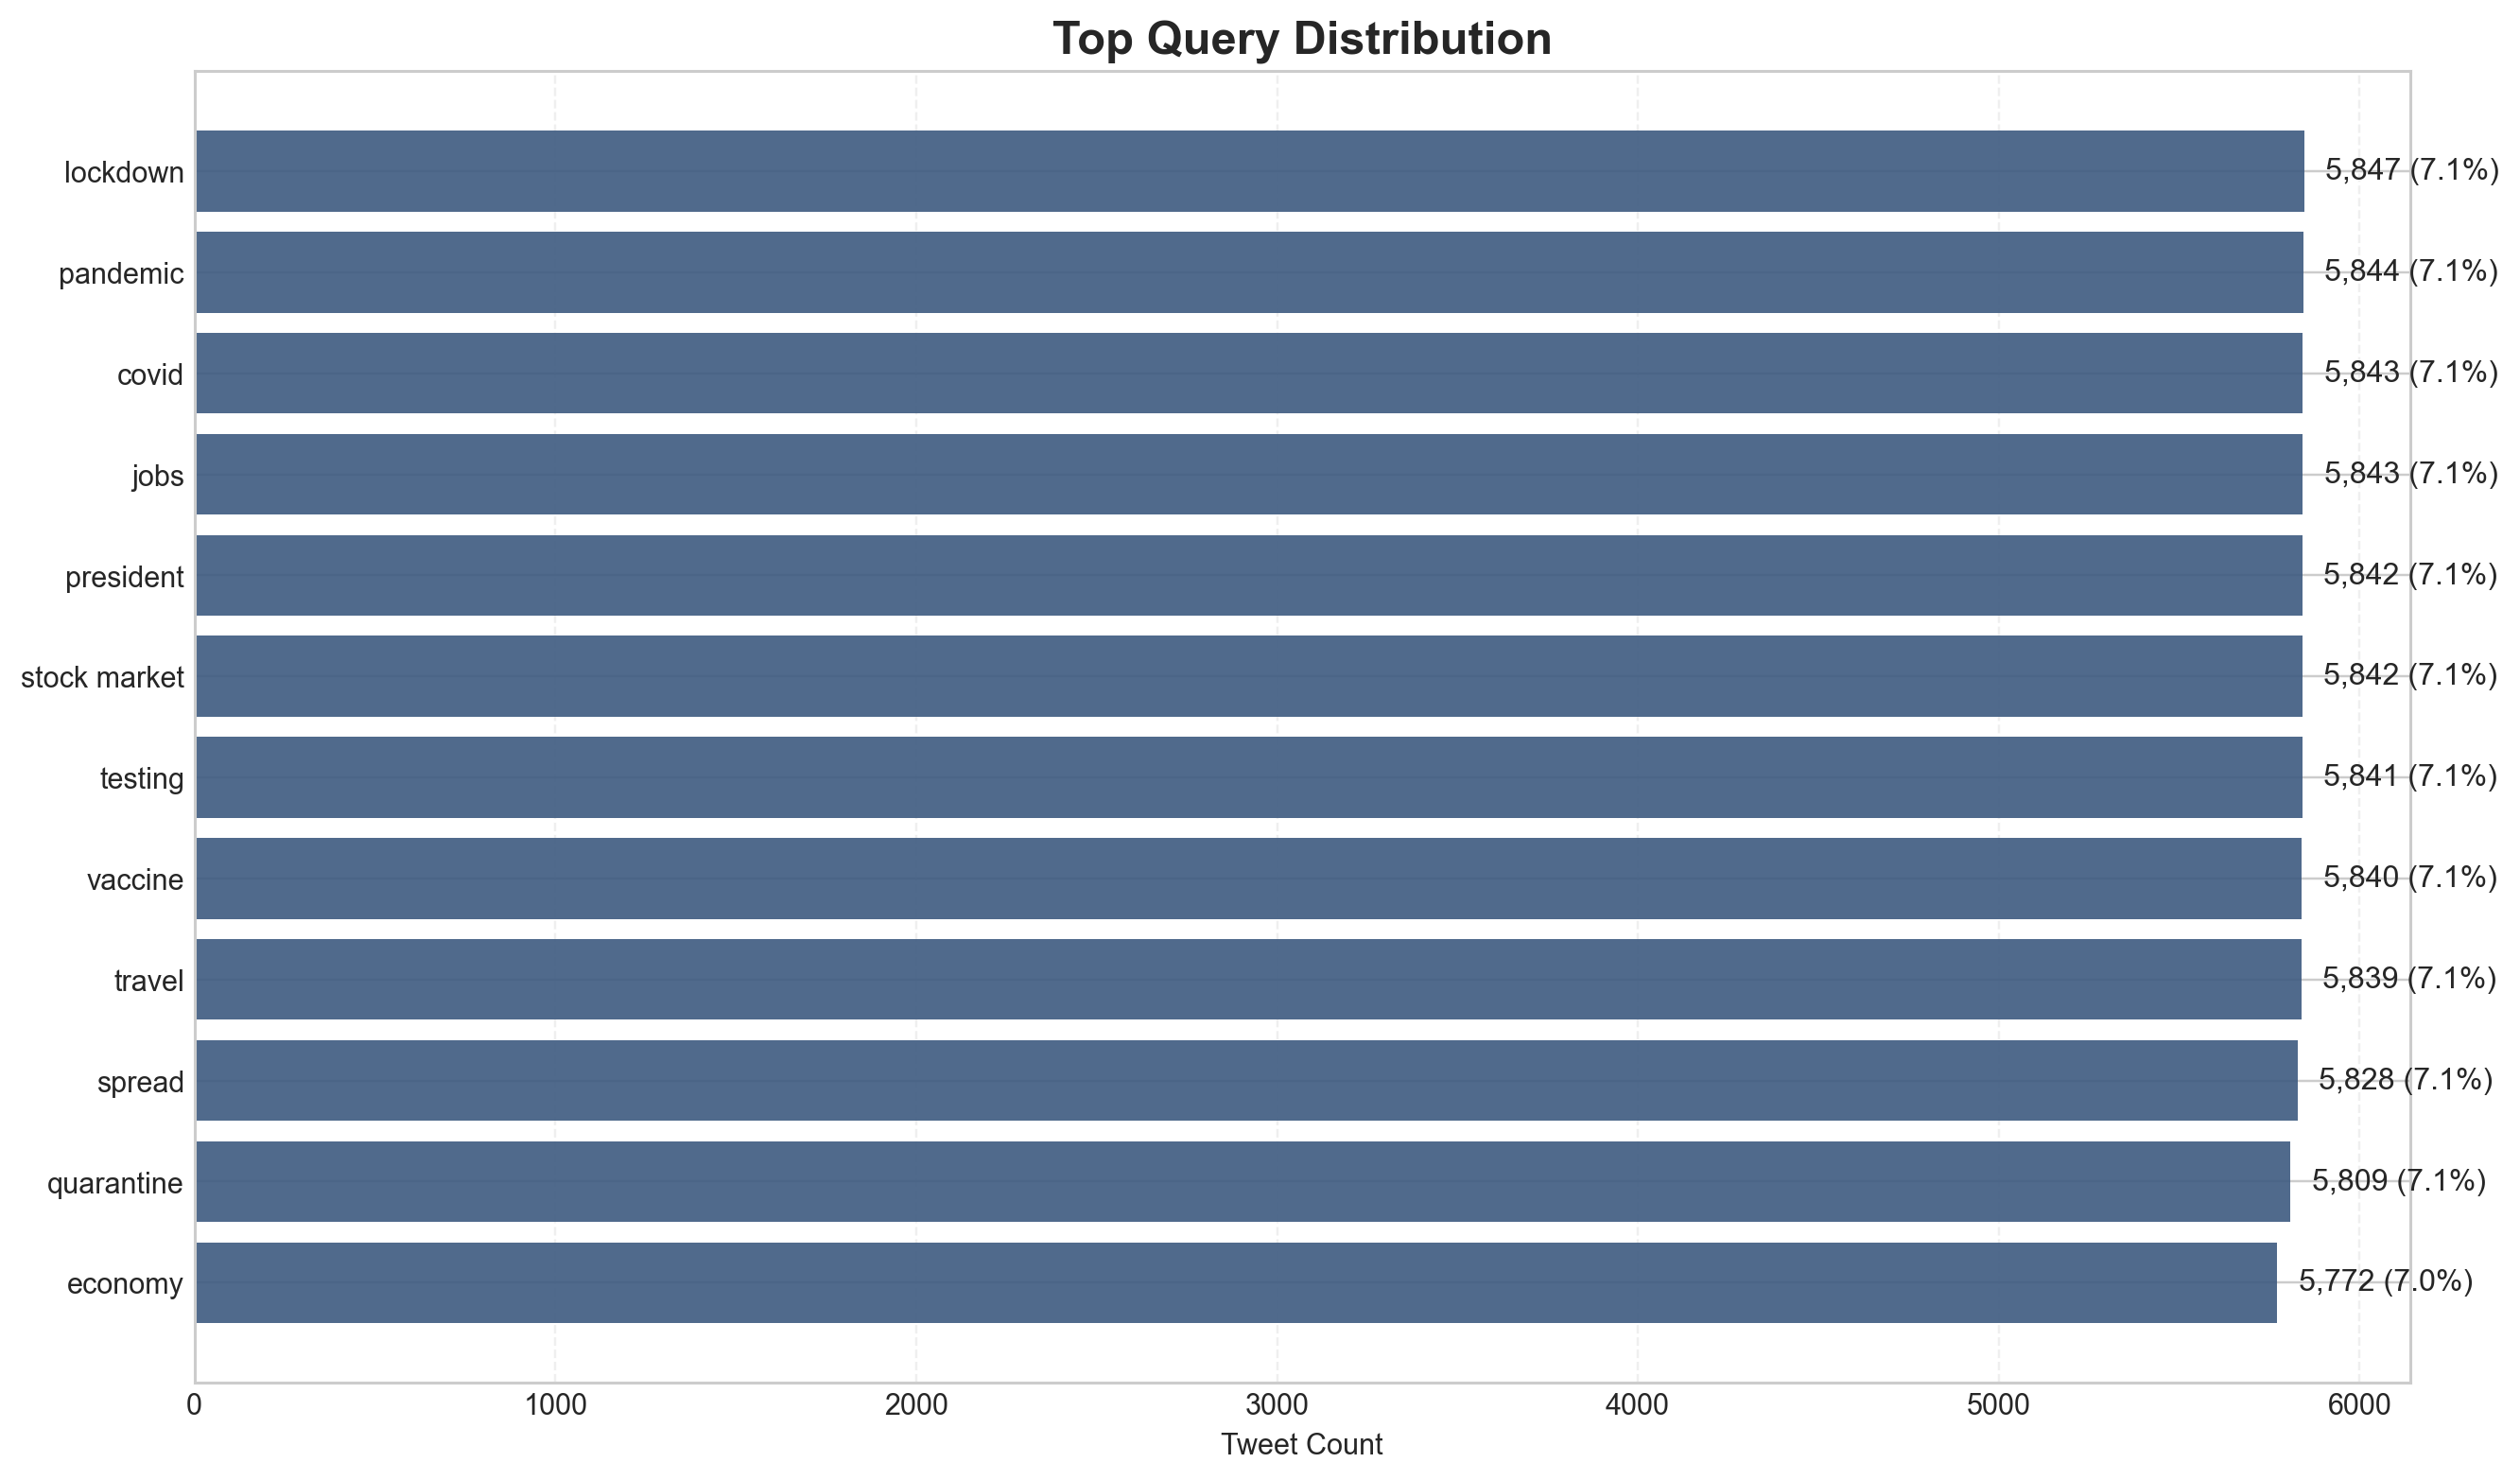
\includegraphics[width=0.90\linewidth,height=0.78\textheight,keepaspectratio]{../outputs/figures/query_distribution.png}
\end{frame}

\begin{frame}{量化摘要與結果解讀}
\begin{columns}[T]
  \begin{column}{0.56\textwidth}
    \begin{tabular}{p{0.48\linewidth} p{0.34\linewidth}}
      \toprule
      指標 & 數值 \\
      \midrule
      有效推文數 & 82,035 \\
      正向比例 & 45.77\% \\
      中立比例 & 20.89\% \\
      負向比例 & 33.34\% \\
      平均情緒分數 & 0.0816 \\
      最繁忙時段 & 13:45 \\
      正向高峰時段 & 13:00 \\
      負向高峰時段 & 09:45 \\
      \bottomrule
    \end{tabular}
  \end{column}
  \begin{column}{0.40\textwidth}
    \begin{block}{結果解讀}
    \begin{itemize}
      \item 整體正向比例高於負向比例。
      \item 不同時段的情緒波動相當明顯。
      \item 資料集屬於多主題混合，因此更適合觀察整體公共討論氛圍。
    \end{itemize}
    \end{block}
  \end{column}
\end{columns}
\end{frame}

\section{結論}

\begin{frame}{專題限制與後續改進}
\begin{columns}[T]
  \begin{column}{0.48\textwidth}
    \begin{block}{目前限制}
    \begin{itemize}
      \item VADER 屬於字典式方法，對諷刺與脈絡理解有限。
      \item 本次資料只涵蓋單日推文，時間跨度較短。
      \item 中英文混雜或特殊語句可能影響判定精度。
    \end{itemize}
    \end{block}
  \end{column}
  \begin{column}{0.48\textwidth}
    \begin{block}{後續方向}
    \begin{itemize}
      \item 導入機器學習或深度學習情緒模型。
      \item 納入多日資料進行事件前後比較。
      \item 加入地區、主題與使用者層級的細部分析。
    \end{itemize}
    \end{block}
  \end{column}
\end{columns}
\end{frame}

\begin{frame}{結論}
\begin{itemize}
  \item 本專題完成了從資料載入、清理、情緒判定到視覺化輸出的完整分析流程。
  \item 程式架構經過模組化整理後，更適合維護與延伸。
  \item 最終成果以圖表與報表雙軌輸出，提升了分析可讀性與簡報展示效果。
  \item 這份專題可作為 Python 資料分析與文字探勘應用的完整案例。
\end{itemize}

\vspace{1em}
\begin{alertblock}{Q\&A}
感謝聆聽，敬請指教。
\end{alertblock}
\end{frame}

\end{document}
